\section{Microsoft Azure}
Microsoft Azure ist kurz gesagt Microsofts Cloud-Plattform, welche seit 2010 angeboten wird. Azure enthält eine laufend wachsende Anzahl an Tools, Diensten, Anwendungen und SQL- sowie NSQL-Datenbanken, die dem Nutzer zur Verfügung stehen. Außerdem bietet es Prozessorleistung und Speicherplatz. Somit erlaubt Azure eben auch das Speichern eigener Daten in der Cloud. Des Weiteren möchte Microsoft damit die IT in Unternehmen flexibler gestalten, denn mit Cloud-Computing lassen sich Infrastrukturen in Form von virtuellen Servern oder Load Balancern digital zur Verfügung stellen. Stichwörter hier sind Ifrastructure-, Platform- und Application-as-a-Service. [1]\\ \\
Grundlage der Azure-Plattform ist dabei ein wachsendes Netzwerk aus Rechenzentren. Damit die Anwendungen überall bereitgestellt werden können, zeigt Microsoft weltweite Präsenz. Es kann dadurch eine enorm hohe Verfügbarkeit gewährleistet werden. Die Sicherung der eigenen Anwendungen und Daten wird durch eben diese Hochverfügbarkeit und eine Notfallwiederherstellung gewährleisten. Laut eigener Aussage wird auch kontinuierlich in die neueste Infrastrukturtechnologie investiert, um zuverlässig, kosteneffizient und vor allem auch umweltverträglich zu bleiben. [1]\\ \\
Derzeit liegt Microsoft noch hinter dem Marktführer Amazon (Quelle Statista). Auf der offiziellen Website von Azure wird die Frage gestellt ‚Azure oder AWS?‘. Microsoft gibt darauf eine selbstbewusste Antwort: ‚Azure ist die richtige Wahl‘.\\ \\ 
Neben der größten Anzahl an Rechenzentren bzw. Regionen in denen diese stehen, bieten sie eine ‚unvergleichliche‘ Hybrid-Cloud. Dies bedeutet, dass Daten und Apps lokal und in der Cloud gespeichert und verknüpft werden können. Zudem bieten sie umfassende Dienste für künstliche Intelligenz, mit die die Entwicklung umfangreicher, intelligenter Anwendungen ermöglicht wird. Nutzer können über Azure auf Hochleistungsgrafikprozessoren zugreifen, wodurch ihnen die Entwicklung im Bereich autonomes Fahren, Spracherkennung sowie Daten- und Videoanalyse erlaubt wird.\\ \\
Azure ist vor allem leicht zu bedienen, zumindest in einer Windows-Umgebung. Vor allem für Windows-Administratoren ist es somit ein Heimspiel. Die übersichtlichen Schritt-für-Schritt-Anleitungen, die dem Anwender zur Verfügung gestellt werden, zeigen, dass die Einrichtung entsprechender Dienste, Server und Cloud-Instanzen sehr leicht ist. Somit macht es den Übergang zur Cloud-basierten Infrastruktur für viele Firmen einfacher. [3] Vor allem das nahtlose Zusammenarbeiten der angebotenen Dienste bzw. Azure-Instanzen erlaubt es sehr leicht eine robuste Infrastruktur aufzubauen. Als Beispiel kann hier der IoT Hub und die sich daran anschließende Ereignisverarbeitung Stream Analytics aufgezeigt werden. [3]\\ \\
Eine Azure-Instanz besteht dabei aus einem virtuellen Server. Dieser wird über Hyper-V (Microsofts Hypervisor zur Visualisierung ihrer Server [4]) betrieben. Kosten fallen anhand der in Anspruch genommenen Leistungen an. Je nachdem, wie häufig Unternehmen ihre Cloud-Instanz verwenden, welche Leistungen und Kapazitäten sie nutzen und vor allem wie viele Daten übertragen werden, was bei Stream Analytics ein wichtiger Faktor ist. [3]\\ \\
Azure erlaubt zudem beliebige Entwicklungstools oder -sprachen. Der Anwender hat die Möglichkeit die Lösung auch mit anderen Tools und Frameworks aufzubauen. 

\section{Azure Stream Analytics}
Wenn man an dem Punkt eines Prozesses angelangt ist, an welchem man eine große Menge von Daten gesammelt und zur Verfügung stehen hat, diese jedoch nur über einen (stark) begrenzten Zeitraum zurückgehalten werden können, bietet Azure Stream Analytics einen Dienst zur weiteren Verarbeitung, welcher nahtlos daran anknüpft. Vor allem im heutigen Industrie 4.0 Umfeld können solche Systeme einen großen Vorteil bieten. Es erlaubt beispielsweise Einblicke in die Sensordaten, um darin nach Mustern zu suchen und entsprechend darauf zu reagieren [1]. Eingehende Daten werden auf Anomalien oder je nach Aufgabe auf relevante Informationen analysiert. Die daraus resultierenden Ergebnisse werden daraufhin entsprechend Präsentiert. Benachrichtigungen werden hier in Echtzeit ausgelöst. Auch auf mobilen Geräten können diese geschickt werden. Ein typisches Echtzeitverarbeitungssystem, welches auf Stream Analytics und weiteren Azure-Diensten aufbaut, wird in Abbildung (…) illustriert.\\ \\
Dieser Service der Azure-Plattform kann Daten aus einem Datenstrom mit hoher Geschwindigkeit bearbeitet. Unterstützt wird dabei eine SQL-Ähnliche Abfragesprache Stream Analytics Query Language (SAQL), über welche man die dynamischen Datenströme analysiert. Diese ist das Herzstück von Azure Stream Analytics. Obwohl SAQL von der allgegenwärtigen SQL-Abfragesprache abgeleitet wurde, enthält es einzigartige Funktionen, die für die Stream-Verarbeitung notwendig sind [6]. Eine dieser Funktionen ist die Möglichkeit, Ergebnisse mithilfe von Zeitfenstern zu erhalten (siehe Fensterfunktionen). \\ \\
Image\\ \\
Die linke Spalte zeigt Sensoren einer IOT-Lösung, Geräte und andere Datenquellen. Diese senden kontinuierlich Daten über das Cloud Gateway an die Azure Hubs [6]. Der Gateway-Dienst ist hierbei ein virtuelles Gerät und ermöglicht eine konsistente und leistungsfähige Verbindung. Die Hubs sind in der Lage Millionen von Ereignissen pro Sekunde zu verarbeiten. Von dort aus werden sie an die weiteren Anwendungen geliefert. Eine Anwendung, um eben diese Daten zu analysieren ist der Stream Analytics-Dienst. Dieser Dienst befindet sich in der Spalte der Transformation. Die Ausgabe kann hierbei auf eine Vielzahl von Endpunkten gerichtet werden. Azure bietet hier einige weitere Dienste, die hier angeknüpft werden können. Die rechte Spalte im Schaubild zeigt lediglich noch die Möglichkeiten, die Daten bzw. Ergebnisse darzustellen [6].\\ \\
Die Eingaben, die ein Stream Analytics-Job benötigt, können einfach im Azure-Portal konfiguriert werden. Eingaben können Azure-Event-Hubs, Azure-IoT-Hubs und Azure Blob-Speicher umfassen. Ein einzelner Stream Analytics-Job kann mehrere Eingaben enthalten. Es können Datenströme zusammengeführt werden, um die kombinierten Daten abzufragen. Dies ist kann mit einem JOIN in SQL verglichen werden. Auch die Ausgaben werden im Portal angegeben. Ausgaben können Kombinationen aus folgenden\\ \\ Komponenten sein:
-	Azure SQL-Datenbank 
-	Azure-Blobspeicher 
-	Azure-Tabellenspeicher 
-	Azure-Ereignis-Hub 
-	Azure-Servicebus-Thema 
-	Azure Service Bus-Warteschlange 
-	Azure DocumentDB 
-	Microsoft Power BI 
-	Azure Data Lake Store 

Diese breite Palette der unterstützten Ausgabetypen, die Azure hier anbietet, ermöglicht eine Menge an Szenarien. Beispielsweise könnten Aufzeichnungen des Stream Analytics-Job in den Azure Blob-Speicher, Azure-Tabellenspeicher, in eine SQL-Datenbank usw. dauerhaft gespeichert werden. Wenn Stream Analytics nun bei der Analyse des Datenstroms Auffälligkeiten oder Anomalien erkennt, können Push-Benachrichtigungen an diverse Geräte gesendet werden. Die Tatsache, dass ein einzelner Stream Analytics-Job mit mehreren Ein- und Ausgängen konfiguriert werden kann, ermöglicht umfangreiche Topologien mit durchgängigen Stream-Processing-Lösungen [6].

\section{Fensterfunktionen}
Eine wichtige Funktion der Stream Analytics-Abfragesprache SAQL ist die Möglichkeit, mit Zeitfenstern zu arbeiten. Ergebnisse werden mithilfe dieser Funktion entsprechend gruppiert. Dies ist vergleichbar mit der GROUP BY-Klausel von SQL mit einer der folgenden Erweiterungen:\\ \\
-	TumblingWindow
-	HoppingWindow
-	SlidingWindow
Beispielsweise soll nun eine Abfrage gestartet werden. Diese soll aufzeigen, wie viele Autos einer speziellen Farbe alle fünf Minuten eine Mautstelle passieren. Mit TumblingWindow kann diese Abfrage so 1:1 implementiert werden. Bei HoppingWindow lässt sich zwar die gleiche Abfrage ausdrücken, allerdings kann hier unabhängig von der Fenstergröße eine Ausgabe erzeugt werden. Es könnte hier beispielsweise einmal pro Minute ausgegeben werden, wie viele Autos einer speziellen Farbe alle fünf Minuten diese Mautstelle anfahren. SlidingWindow hingegen lässt die Abfrage zu, in welchen 5-Minuten-Zeitfenstern zehn oder mehr Autos einer speziellen Farbe die Mautstelle erreichen. SlidingWindow ist somit für den Umgang mit relativ spärlichen Ergebnismengen geeignet. Diese Konzepte sind in Abbildung 3 dargestellt [6].\\ \\
Image

\section{Lambda-Architektur}

\begin{quote} \textit{\glqq Mithilfe des Lambda-Architektur-Konzepts haben wir eine Architektur geschaffen, für die immer stärker wachsende Datenberge und neue Anforderungen der Zukunft kein Problem darstellen. \grqq~}\cite[S.2]{opitz.2017} \\ \end{quote} 
Bei der Verarbeitung von Big Data entstehen Herausforderungen wie z. B. die Echtzeitverarbeitung und die Hohe Rechenkomplexität. Um diese Herausforderungen zu bewältigen wird eine Big-Data-Architektur benötigt, welche eine geringe Latenz zwischen Ein- und Ausgabe aufweist. In diesem Kontext wird die Lambda-Architektur erwähnt, welches in Stream Analtics Einsatz findet \cite{Familiar.2017}.Die  Lambda-Architektur ist ein bekanntes Big-Data-Pattern und beschreibt den  konzeptionellen  Aufbau  einer  Big-Data-Architektur bestehend  aus  einem  zentralen  Eintrittspunkt. Diese besteht aus zwei Kernschichten: Batch- und Speed-Layer. Die Vereinigung dieser Schichten führt zu einer Echtzeitübermittlung der Daten. Die Umsetzung der Lambda-Architektur erfolgt in vielen Fällen nicht in reiner Form. die Systemlandschaft sieht zwar aus wie bei eine Lambda-Architektur, allerdings ist die Interaktion der Komponenten anders, da beispielsweise verschiedene Anwendungsfälle unterschiedliche Schwerpunkte haben.  \\ \\ \textbf{Speed Layer}. Sie hat die Aufgabe möglichst aktuelle Daten zu liefern. Dabei wird nicht auf Datenvollständigkeit und -korrektheit geachtet, da die Datenmenge bei so einer hohen Frequenz nicht vollständig verarbeitet werden können bzw. dies nicht zwanghaft notwendig ist. Beispielsweise ein Sensor, der in Millisekunden abständen die Raumtemperatur verschickt. Hier könnte auch jeden tausendsten Sensorwert verarbeitet werden, da der Nutzwert von mehreren Daten an dieser Stelle nicht gegeben ist. Hier geht es darum, dass die Verzögerungslücke, welches von der Stapelschicht verursacht wird, zu minimieren. Die Verarbeitung der Daten geschieht im besten Falle komplett „in-Memory“.\\ \\ \textbf{Batch Layer}. Sie bezieht alle Daten ein und achtet darauf, exakte Ergebnisse zu erbringen. Im Gegensatz zu dem Speed Layer muss die Daten nicht im Speicher halten und kann Analysen mehrere Zeitfenster hinweg durchführen. Beispielsweise wäre ein Trainingsmodell aus dem Bereich „Machine Learning“ ein Anwendungsfall, welches Microsoft Azure ebenfalls unterstützt \cite{Berle.2017}. 

\begin{figure}[h!]
	\centering
	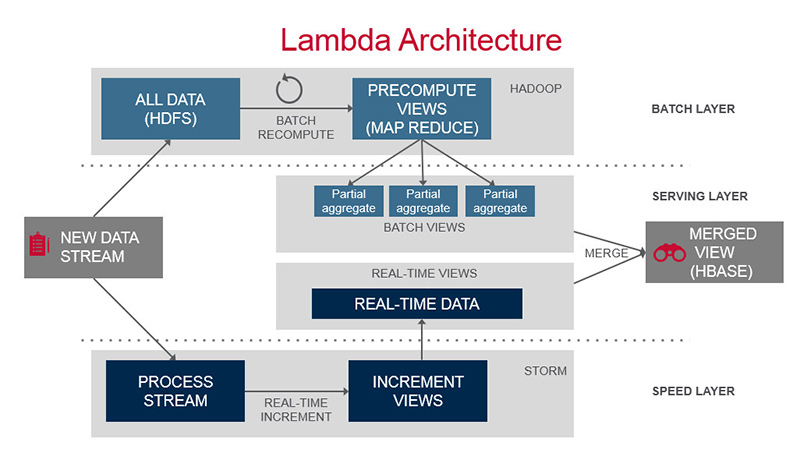
\includegraphics[width=1.0\linewidth]{images/lambda-architecture}
	\caption{Aufbau der Lambda-Architektur} %Generelle
	\label{fig:cnn_structure}
\end{figure}